\documentclass[conference]{IEEEtran}
\IEEEoverridecommandlockouts
% The preceding line is only needed to identify funding in the first footnote. If that is unneeded, please comment it out.
%\usepackage{cite}
\usepackage{amsmath,amssymb,amsfonts}
\usepackage{algorithmic}
\usepackage{graphicx}
\usepackage{textcomp}
\usepackage{xcolor}
\def\BibTeX{{\rm B\kern-.05em{\sc i\kern-.025em b}\kern-.08em
		T\kern-.1667em\lower.7ex\hbox{E}\kern-.125emX}}

\usepackage{hyperref}
\usepackage{biblatex} 
\addbibresource{references.bib}

% To get bulletpoints inside a table cell
\usepackage{array}

% All images go in folder below
\graphicspath{{./pix/}} % put all your figures here.

\begin{document}
	
	\title{Recognizing Activities of Daily Living Using Audio and IMU Data from Commodity Smartwatches
	}
	
	\author{
		\IEEEauthorblockN{Yvette Espinoza}
		\IEEEauthorblockA{\textit{Department of ECE} \\
			\textit{Purdue University}\\
			Los Angeles, CA \\
			yespinoz@purdue.edu}
		
		\and
		\IEEEauthorblockN{Cameron Johnson}
		\IEEEauthorblockA{\textit{Department of ECE} \\
			\textit{Purdue University}\\
			Asheville, NC \\
			john3096@purdue.edu}
		
		\and
		\IEEEauthorblockN{Jahangir Mollah}
		\IEEEauthorblockA{\textit{Department of ECE} \\
			\textit{Purdue University}\\
			Seattle, WA \\
			jmollah@purdue.edu}
	}
	
	\maketitle
	
	\begin{abstract}
		Human activity recognition is applicable to many fields, such as healthcare, but there are limitations on devices that can be used.
		The popularity of smart devices allow for comfort while also providing the data necessary to enable activity recognition.
		Smart watches prove especially practical for recording both acoustic and inertial data because the mic is at close proximity to the hand which is often close to the activity being performed. The IMU records useful motion on the wrist as opposed to a smartphone in the pocket or strapped to the chest.
		This project builds on previous activity recognition research and focuses on the effects of acoustic and motion noise on recognizing the activities of daily living.
		
	\end{abstract}
	
	%\begin{IEEEkeywords}
	%component, formatting, style, styling, insert
	%\end{IEEEkeywords}
	
	\section{Introduction}
	
	Early research in activity detection aimed at finding differences in signal characteristics of the collected accelerometer data, and determining the ideal sensor placement. 
	In \cite{2011_Sensor_Positioning}, activities were grouped together into four categories by levels of physical activity, and sensors were placed throughout the body to determine the best location for each of the categories.
	Their results found each category performed best with a different sensor location. A sensor placed on the waist was best at detecting low level activities like eating, while a sensor on the chest or wrist was best at medium level activities like housework.
	
	While different sensor placement based on an activity would be ideal for performance, it would not be practical for widespread use.
	An accelerometer by itself is not enough to determine an activity. More context is needed and different sensors on the body are an inconvenience for users. 
	Human activity recognition is widely used in healthcare applications, with the elderly being a large part of the user demographics \cite{2018_Robust_Activity}, to suit their needs the data collection would require an unobtrusive setup.
	To address the inconvenience of full body sensors and the need for context, \cite{2012_WristSense} used a wrist-worn device equipped with an accelerometer and camera to recognize daily activities. 
	The camera provided context for the activities, and the accelerometer provided characteristics of the body movement associated with different activities, both of which were used to train a model to predict the activity.
	
	The advancement in smart devices, like smartwatches and conversational assistants, allow for more sensors in a user friendly device.
	Conversational assistants, like a Google Home, and smartwatches are used to train a model to recognize activities of daily living \cite{2021_Ok_Google} \cite{2022_Leveraging_sound}.
	
	%\subsection{Machine Learning Algorithms}
	% TODO - talk about the machine learning advances --> smart devies allow for more data collection, which allow for better ML models and classifiers %
	
	\subsection{Applications}
	Audio monitoring can also be used to detect hazardous situations such as loud noises, falls, or emergencies. By integrating audio analysis into a smartwatch, users can be alerted to potential dangers in real-time, providing an added layer of safety.
	
	Human activity recognition has potential applications that can be leveraged in healthcare, dietary monitoring, and weight management.
	One application is to provide a user with a more holistic view of their lifestyle, providing details on how long they spend on activities such as cooking or browsing on a phone. This information can be used to reflect and better manage time.
	Another important application is for monitoring the progress of debilitating medical conditions, such as cognitive impairment.
	
	We propose expanding on research recognizing activities of daily living using the IMU and audio data from a commodity smartwatch. 
	We will be following existing research performed in \cite{2022_Leveraging_sound}, but adding extra noise while collecting data to better understand the effects of such noise in recognizing activities.
	
	\subsection{Motivation}
	The researchers of the original paper conducted two generally different experiments. In the first experiment, referred to as the semi-naturalistic experiment, an individual performs a series of activities for 30 seconds wearing a Fossil smartwatch which records inertial and acoustic data. There is a clear distinction between each activity and the watches are programmed to listen at frequent intervals. The authors implemented a variety of machine learning models to recognize the activity in this experiment with an accuracy of 94.3 \%. The second experiment, referred to as the in-the-wild experiment, implements a less controlled, more realistic setting.
	One limitation of this paper was that their uncontrolled experiment had poor results due to background noise, mislabeling of activities due to the setup, and inconsistencies in how activities were performed.
	Since their in-the-wild experiment was not controlled, not all the activities they were interested in were performed, in some cases activities overlapped, and combined with a limited sample size resulted in misclassifications \cite{2022_Misclassifications}.
	
	The goal for this project is to expand on the previous work and better understand some of the limitations the researchers encountered.
	Since the main limitation was the performance degradation for their in-the-wild study, this project aims to have a semi-controlled environment, or semi-wild experiment, where activities are pre-defined but the noise from the in-the-wild study is added. 
	The following are the areas of interest: measure the effect of wearing the watch on a passive instead of dominant hand, measure the effect of background noise while performing activities, and determine if more participants would lead to more accurate results.
	
	\section{Related Work}
	\subsection{Sound Classification}
	A recent survey of hard of hearing people found that smartwatches, instead of smartphones, are the preferred device for sound awareness due to their social acceptability and support for both visual and haptic feedback \cite{2020_SoundWatch}.
	Due to this demand, smartwatches are becoming more popular in sound classification research, but there are still limitations on performance due to acoustic variations, or background noise.
	
	One study measured the effect of background noise on speech detection and found that a noisy environment caused performance to drop by about 20 \% \cite{2002_Content_Analysis}.
	Their proposed solution to the performance degradation was to use new features, which did improve performance.
	
	Other studies suggested having a user-centred data collection, where the user would record the same activity of interest in different scenarios, which would then be used to train a model to detect that activity \cite{2016_Personalizable} \cite{2020_SoundWatch}.
	
	\subsection{Motion Classification}
	There was also a study done where work proposes several techniques to improve the robustness of a Human Activity Recognition (HAR) system that uses accelerometer signals from different smartwatches and smartphones. When using smartwatches to recognize whole body activities, the arm movements introduce additional variability giving rise to a significant degradation in HAR\cite{2018watch_martphone}
	
	Other research was done using Samsung Gear Smartwatch to collect data, then extract features, classify with H-SVM (Hierarchical Support Vector Machine) classifier and identify human activities classification. Experiment results show great effect at low sampling rate, such as 10 and 5 Hz, which will gives the energy saving. In most cases, the accuracy of activity recognition experiments was above 99 percent\cite{2017_SVM}
	
	\section{Machine Learning models}
	Classical machine learning models such as Random Forest, Naive Bayes, and AdaBoost have been used in previous studies and prove to be effective in human activity recognition, but they rely on heuristic handcrafted feature extraction. These models showed decent results, but accuracy was only in the range of 60 to 85 for classifying motion data and 40 to 70 when classifying audio data. In order to achieve more reliable classification, the authors of \cite{2022_Leveraging_sound} experimented with two different deep neural network models and tried different fusion methods of the acoustic and motion data. These deep human activity recognition models allow input of raw sensory data captured by the smart watch instead of relying on expensive, handcrafted feature extraction and showed significant improvement to accuracy. The motion and acoustic data are trained separately using different models and then fused using a variety of techniques.
	
	\subsection{Inertial Model}
	Two different models were experimented with to classify the inertial data. One of the models used is a variation of a framework called DeepConvLSTM which is based on convolutional and LSTM recurrent units. The modification allows the model to extract accelerometer and gyroscope features separately and then concatenate each modality at the last layer before passing through the softmax classifier. This modification improved accuracy, but the other model which was used, called Attend and Discriminate, proves to be more effective. This framework incorporates cross-channel self-attention and temporal attention. Both gyroscope and accelerometer data are concatenated before processing through convolutional layers to learn the interaction between the two. The resulting feature maps pass through a recurrent neural network to model temporal dynamics.
	
	\subsection{Acoustic Model}
	In order to classify the acoustic data, the audio clips required some pre-processing. Log-mel spectrograms are extracted from the clips by computing the short-time Fourier transform for each segment, using a Hanning window of 1024 samples and hop size of 320 samples, and then converted into a 64-bin log-scalled Mel spectrogram.  Convolutional neural networks are applied to these log-mel spectrograms. The authors find a CNN architecture they refer  to as CNN14 comprised of six convolutional blocks consisting of two convolutional layers and intermediary average pooling layers.
	
	\begin{figure}[h]
		\centering
		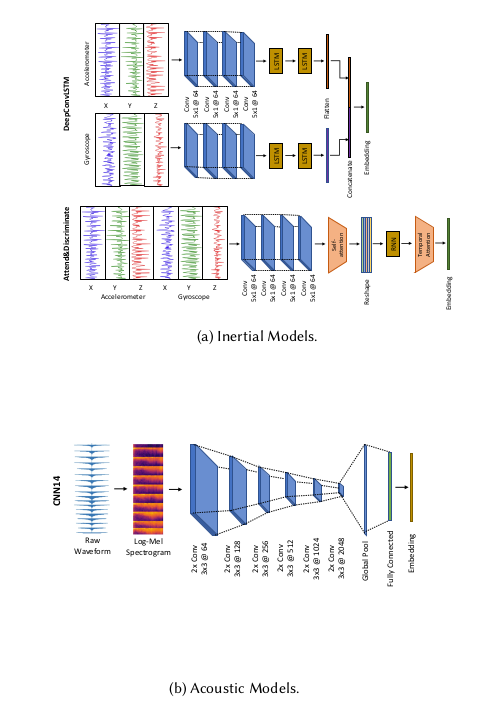
\includegraphics[scale=0.50]{Architecture_of_Inertial_and_Acoustic_Models}
		\caption{Architecture of Inertial and Acoustic Models, provided by \cite{2022_Leveraging_sound}}
		\label{fig: Architecture_of_Inertial_and_Acoustic_Models}
	\end{figure}
	
	\subsection{Fusion Methods}
	The inertial and acoustic data then need to be incorporated together. The model applies an aggregation method which concatenates the feature maps. There were other methods such as score-level fusion, but they did not perform as well. The concatenated feature maps are followed by a single classification head and joint training of both acoustic and inertial networks. The predicted class probabilities are averaged for a final probability value.
	
	\section{Methodology}
	For the data collection, only a subset of the original activities was performed: writing, typing on a keyboard, brushing teeth, sweeping, and washing dishes.
	These activities were selected since they primarily rely on one measurement for detection, i.e. washing dishes is more easily identified by its acoustic data while writing is more identifiable by its motion data.
	A smartwatch was worn to collect the accelerometer and gyroscope data \cite{2020_Accelerometer_and_Gyroscope}, while a phone was set nearby to collect the acoustic data.
	The motion and acoustic data were the inputs to a deep learning model which fuses the inertial data and acoustic data to determine the activity being performed, shown in Figure \ref{fig: Architecture_of_Inertial_and_Acoustic_Models}.
	
	\subsection{Hardware Setup}
	In the original paper the authors used the same watch, the Fossil Gen 4, for all of their experiments \cite{2022_Leveraging_sound}.
	Their custom application, which collected motion and acoustic data, was developed on Android Wear OS 2.11, with inertial sampling at 50 Hz and acoustic sampling at 22.05 kHz.
	
	For this project, two separate Samsung Galaxy watches were used with a custom app developed on Tizen OS 5.5.
	The inertial data was also sampled at 50 Hz, but since the smartphone recorded at 44.1 kHz, it was downsampled in post processing to match the rate of the original paper.
	
	\subsection{Watch App}
	The original intention was to collect both motion and acoustic data from the smartwatch, but while developing the app there were problems with writing to the watch's file system.
	The main problem seemed to be with the permissions configured on the native c app.
	Based on the available documentation, those problems could be addressed by switching to a web app instead, but due to lack of experience with web apps and time constraints, instead of storing the collected data to a file on the watch the inertial data was collected from the debug log and a smartphone was used to collect the acoustic data.
	
	The final app only had one button to start and stop the motion data collection, shown in Figure \ref{fig: watch_app_picture}.
	
	\begin{figure}[h]
		\centering
		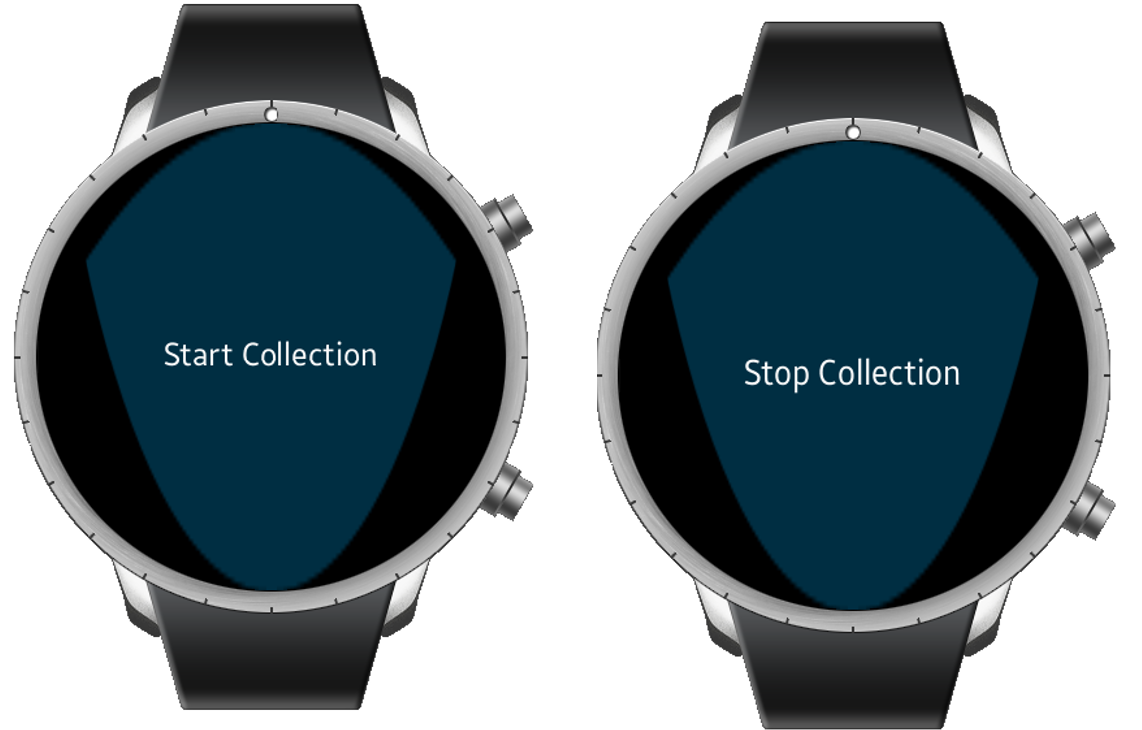
\includegraphics[scale=0.75]{watch_app_picture}
		\caption{Watch app deployed on emulator}
		\label{fig: watch_app_picture}
	\end{figure}
	
	\subsection{Schedule}
	The project was divided into four phases.
	More details on due dates and deliverables for each phase are provided in Table \ref{tab: Schedule}.
	
	\begin{table}[htbp]
		\caption{Schedule}
		\begin{center}
			\begin{tabular}{| m{1.2cm} | m{4cm} | m{1.2cm} |}
				\hline
				\textbf{Phase} & \textbf{Activities} & \textbf{Due Date} \\
				\hline
				Planning & 
				\begin{itemize}
					\item Identify existing research data
					\item Identify available hardware
					\item Plan for how to capture and store data
					\item Identify how to process data
					\item Identify machine learning classification models
				\end{itemize} &
				March 18 \\
				\hline
				
				Data Collection & 
				\begin{itemize}
					\item Capture and process raw data
					\item Capture audio data at all times
					\item Review existing research data
					\item Get volunteers for experiments
				\end{itemize} & 
				April 1 \\
				\hline
				
				Analysis & 
				\begin{itemize}
					\item Fuse data collected from different sources
					\item Label data collected
					\item Run the classification models
					\item Analyze results
				\end{itemize} & 
				April 15 \\
				\hline
				
				Finalize Report & 
				\begin{itemize}
					\item Write up final report
					\item Create presentation
				\end{itemize} & 
				May 6 \\
				\hline
			\end{tabular}
			\label{tab: Schedule}
		\end{center}
	\end{table}
	
	\section{Data Collection}
	The data collection was performed using a debug version of the watch app, which allowed us to access the debug log with the accelerometer and gyroscope data.
	Participants had two data collection sessions.
	For the first session the watch was worn on the dominant hand and there was no background noise, and for the second session either the watch was worn on the passive hand or background music was played while performing the activities.
	A phone was placed next to the participant during data collection to capture the activities acoustic data.
	Figure \ref{fig: data_collection_steps} shows the instructions for how to collect data. 
	Figure \ref{fig: DeviceManager} shows the Tizen Device Manager from which the debug log was exported.
	
	\begin{figure}[h]
		\centering
		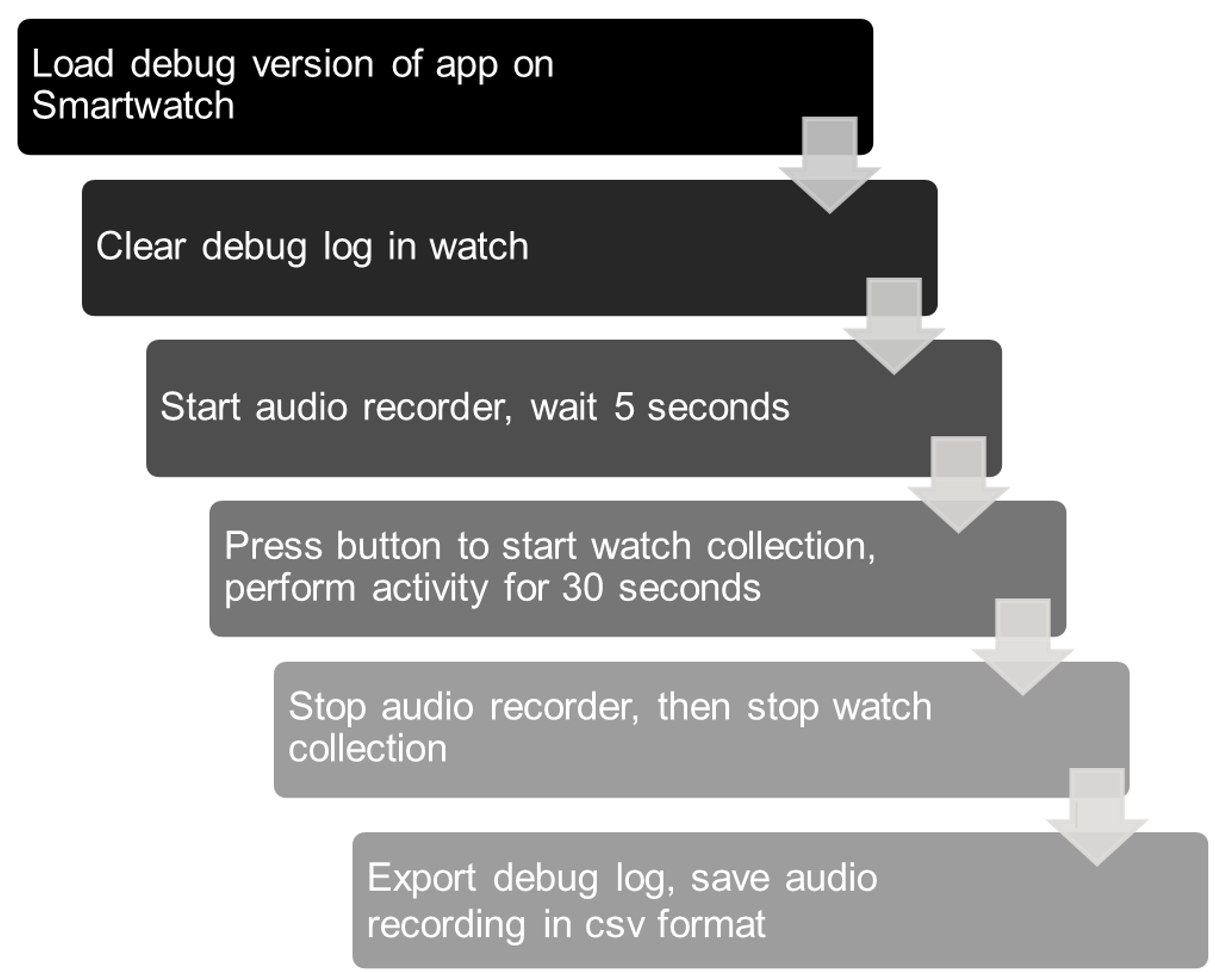
\includegraphics[scale=0.70]{data_collection_steps}
		\caption{Data collection steps provided to the participants}
		\label{fig: data_collection_steps}
	\end{figure}
	
	\begin{figure}[h]
		\centering
		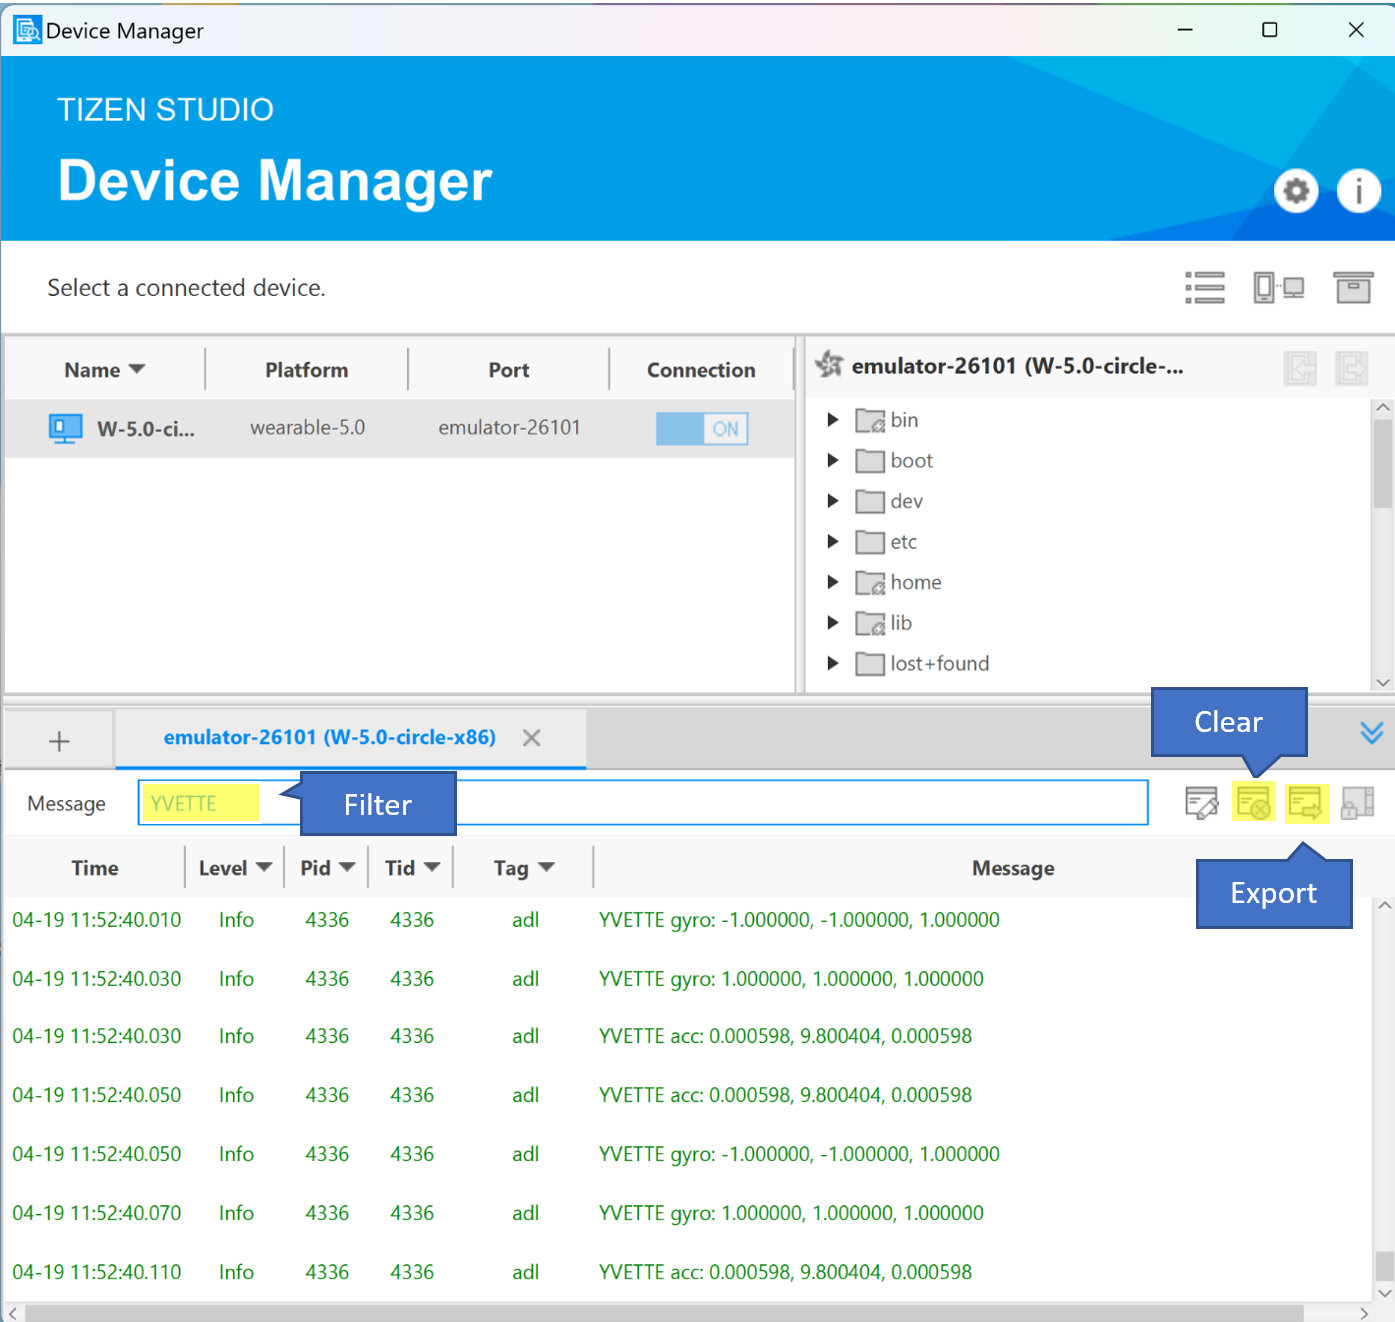
\includegraphics[scale=0.60]{DeviceManager}
		\caption{Example of how to clear and export the debug log}
		\label{fig: DeviceManager}
	\end{figure}
	
	\subsection{Data Post-processing}
	To align the acoustic and inertial data, the first and last 5 seconds of the audio file were removed.
	The next step was to downsample the recordings, since the smartphones sampled at 44.1 kHz while the original paper sampled at 22.05 kHz.
	For the inertial data, the debug logs were parsed and only timestamps that collected both gyroscope and accelerometer data were used to generate the final csv.
	
	The final step was to rename the files and add them to the same file structure as used by the original researchers.
	Since only a subset of the original activities were performed, audio and motion data from other participants were used to create a full activity set that would be ready to test the models pre-trained on the available datasets.
	
	\section{Results}
	\subsection{Running the original models}
	Although the machine learning models are publicly available, they required significant modification. The reason for these changes are mostly due to using different equipment. In order to increase our compute power, we tailored the model to use Google Colab which can run independently from our machines and employs more powerful hardware. In doing so, the pre-processing and training methods were still crashing due to insufficient memory. Specifically, the program stacked the audio and inertial data for all participants into arrays using a numpy method which required keeping the entire array in memory. We reconfigured the code to use numpy views to combine all of the data which proved much more efficient and ultimately cut the memory requirement in half.
	Other modifications to the model included changing plotting methods and various function parameters most likely due to the authors employing outdated libraries.
	
	\subsection{Number of participants}
	We wanted to verify whether adding more training data was likely to improve the accuracy of the model. To do this, we ran the model using different numbers of participants and recorded the final test accuracy to evaluate whether the improvement starts to decrease. Figure \ref{fig: f-score_vs_participants} shows the results of this experiment after training for 100 epochs. As you can see, training on just two participants performs poorly with an accuracy of around 40 percent. If you run the same experiment using more participant data, the accuracy improves significantly. Importantly, the upward trend shows no sign of leveling. The plot suggests that including more training data will further improve the model accuracy. 
	Figure \ref{fig: Original_Confusion_Matrix} shows the confusion matrix for the original model trained on all the available semi-naturalistic data. The model performs well, but there is still room for improvement.
	
	\begin{figure}[h]
		\centering
		\includegraphics[scale=0.60]{fscore_num_p.png}
		\caption{F-score for training on increasing amount of participants}
		\label{fig: f-score_vs_participants}
	\end{figure}
	
	\begin{figure}[h]
		\centering
		\includegraphics[scale=1.2]{Original_Confusion_Matrix}
		\caption{Confusion matrix for model trained on Semi-Naturalistic dataset}
		\label{fig: Original_Confusion_Matrix}
	\end{figure}
	
	\subsection{Inference on trial data}
	To better define the data collection process a trial run was conducted where only three activities were performed: writing, typing and wiping the table.
	Each data collection lasted 15 seconds, and motion data was sampled at 10 Hz instead of 50 Hz as in the original paper.
	After post-procesing, the data was fed into a model that was pre-trained with the original dataset, the model output is shown in the Figure \ref{fig: Our_data_inference} confusion matrix.
	
	\begin{figure}[h]
		\centering
		\includegraphics[scale=0.70]{Our_data_inference}
		\caption{Confusion matrix for trial data run from model trained with semi-naturalistic dataset}
		\label{fig: Our_data_inference}
	\end{figure}
	
	On the confusion matrix the left side indicates the input activity, and the bottom shows the predicted activity, with the three activities performed highlighted: writing (A), typing (D), wiping table (J). 
	The activities were all labeled incorrectly, writing and typing were mistaken for brushing hair (K) and wiping table was mistaken for scratching (I).
	After reviewing the results, the collection time was increased to 30 seconds, and the motion sampling rate was changed to 50 Hz. 
	Due to time constraints the updated collection procedure was not able to be tested.
	
	\section{Challenges}
	There were three main challenges encountered while working on this project. 
	\subsection{Activity Selection}
	The first challenge was selecting the reduced activity list to analyze for the project.
	The original motivation behind the project was to apply the models and focus on detecting digital media usage, which is one of the applications for activity detection. 
	Previous research showed the controlled environment results were accurate in detecting the different activities, but we found our semi-wild results were similar to the uncontrolled results, where differentiating between the different phone activities, typing on the phone and browsing on the phone, was difficult.
	The focus then became measuring the effect of noise that was causing the degraded performance between the controlled and uncontrolled experiments. Our motivation focused on testing with Motion noise and acoustic noise and evaluating the performance of the model.
	
	
	\subsection{Data Collection}
	The app development was a major challenge, mostly because none of the team members had any app development experience.
	As previously mentioned, the original plan was for the watch to collect and locally store both acoustic and inertial data, and the files would later be moved from the watch to a computer.
	The older Samsung watches that were used had Tizen OS, and because it is not as popular as WearOS, there was a lack useful documentation while attempting to troubleshoot.
	Tizen OS has been replaced by WearOS in the newer Samsung watches, so future research shouldn't have these same problems.
	
	\subsection{Running the original models}
	The original models had to be modified before they could be used. 
	Due to their complexity and memory requirements, only one member was able to get them to fully run. This was only after tailoring the model to run on Google Colab because none of us had the necessary hardware, specifically the memory and GPU processing. Even with upgrading to high-ram and GPU processing through Colab, the model required over five hours to train using 15 participants. Fortunately, we were able to save the weights after each training session which allowed the other members to continue work, but there was that added delay before more analysis could be conducted.
	
	\section{Conclusion}
	
	We were able to incorporate the data from the 15 participants whom the authors used to gather data performing various activities around the house. Using the Attend and Discriminate-CNN14 model and concatenating the acoustic and inertial data, we achieved fairly reliable results classifying human activities. Our preliminary results indicate that including more participant data will continue to improve accuracy. Given more time, we would have liked to experiment with more data and recording data in various noisy environments with factors such as dog barking or music in the background.
	
	
	\section*{Acknowledgment}
	We re-implemented the following paper using their available models and datasets: \cite{2022_Leveraging_sound}.
	
	\nocite{*}
	\printbibliography
	
\end{document}
